\documentclass{article}

% Подключение пакетов, если необходимо
\usepackage[utf8]{inputenc}
\usepackage[T1]{fontenc}
\usepackage[russian]{babel}
\usepackage{graphicx}

% Начало документа
\begin{document}

% Титульная страница
\title{Название документа}
\author{Автор}
\date{\today} % или указать конкретную дату

\maketitle

% Содержание документа
\section{Введение}
Текст введения...

\section{Заголовок раздела}
Текст вашего раздела.

\subsection{Подраздел}
Текст вашего подраздела.

\begin{itemize}
  \item Элемент списка 1
  \item Элемент списка 2
\end{itemize}

\begin{table}
  \caption{Заголовок таблицы}
  \begin{tabular}{|c|c|}
    \hline
    Заголовок столбца 1 & Заголовок столбца 2 \\
    \hline
    Значение 1 & Значение 2 \\
    \hline
  \end{tabular}
\end{table}

\begin{figure}
  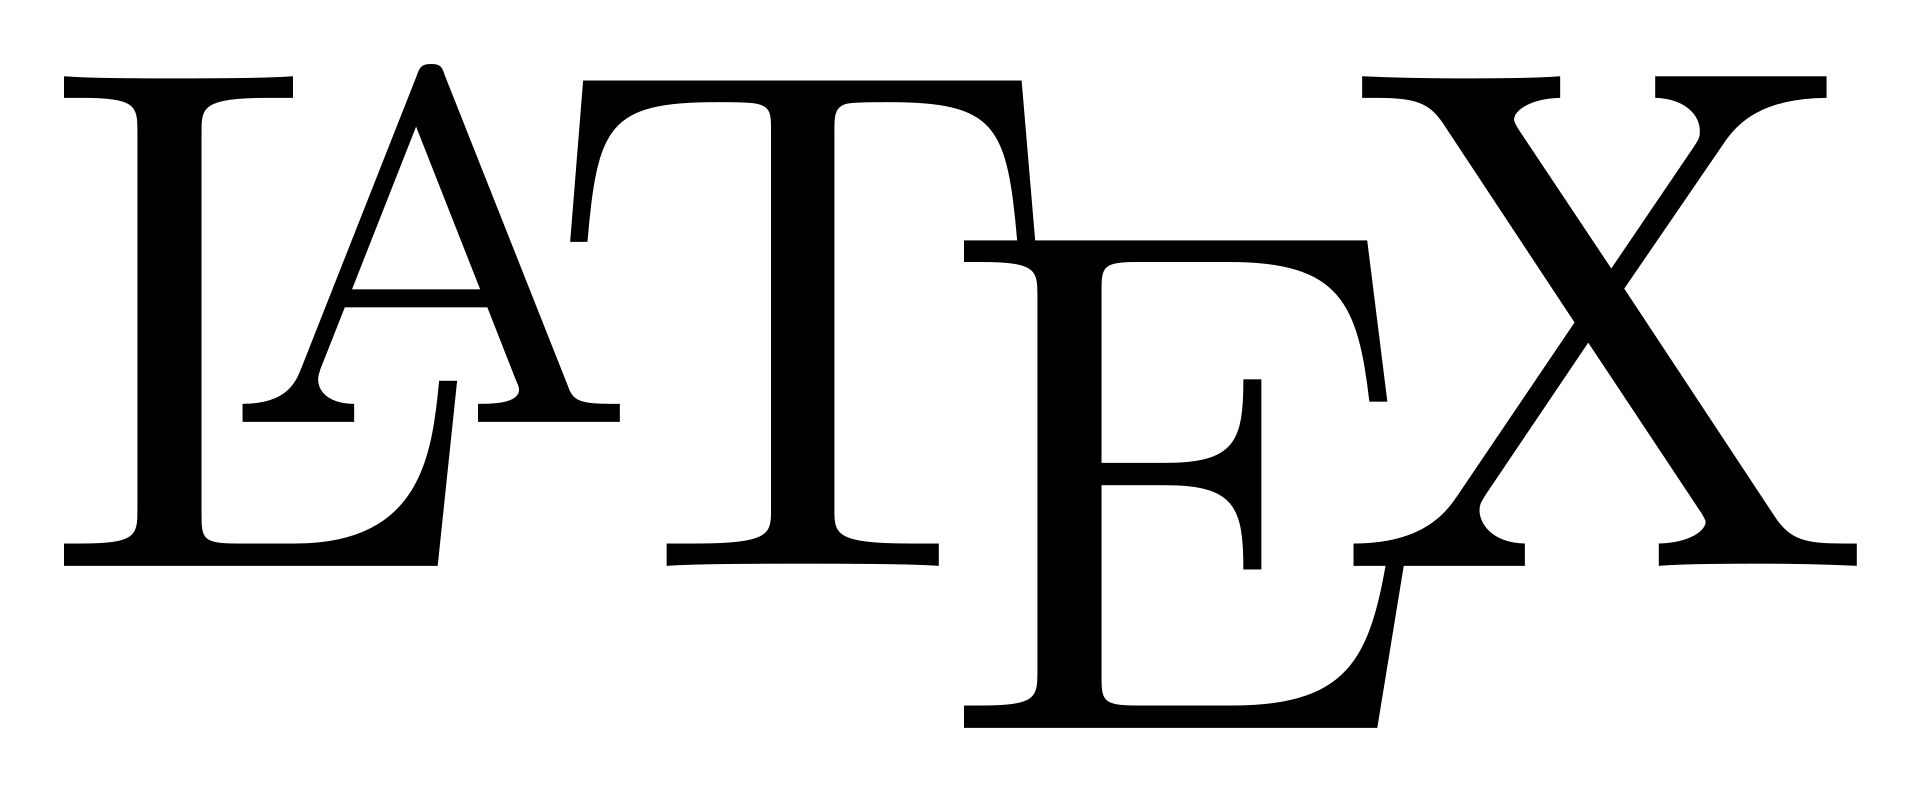
\includegraphics[width=\textwidth]{your-image.png}
  \caption{Подпись к изображению}
\end{figure}

\section{Заключение}
Текст заключения...

%Список использованных источнико
\begin{thebibliography}{99}
   \bibitem{...}
   ...
 \end{thebibliography}

% Приложения
 \appendix
\section{...}

% Конец документа
\end{document}